\textbf{Partie 1}

\medskip

Soit $g$ la fonction définie pour tout nombre réel $x$ de l'intervalle $\intervOO{0}{+\infty}$ par : \[g(x) = \dfrac{2 \ln x}{ x}.\]
%
\begin{enumerate}
	\item On note $g'$ la dérivée de $g$. Démontrer que pour tout réel $x$ strictement positif : \[g'(x) = \dfrac{2 - 2\ln x}{x^2}.\]
	\item On dispose de ce tableau de variations de la fonction $g$ sur l'intervalle $\intervOO{0}{+\infty}$ : 
	
	\begin{center}
		\begin{tikzpicture}[double distance=4pt]
			\tkzTabInit{$x$/0.8,$g$/2.4}{$0$,,$\e$,$+\infty$}
			\tkzTabVar{D-/$-\infty$,R,+/$\dfrac{2}{\e}$,-/$0$}
			\tkzTabVal{1}{3}{0.5}{1}{$0$}
		\end{tikzpicture}
	\end{center}
	
	Justifier les informations suivantes lues dans ce tableau:
	
	\begin{enumerate}
		\item la valeur $\dfrac{2}{\text{e}}$ ;
		\item les variations de la fonction $g$ sur son ensemble de définition ;
		\item les limites de la fonction $g$ aux bornes de son ensemble de définition.
	\end{enumerate}
	\item En déduire le tableau de signes de la fonction $g$ sur l'intervalle $\intervOO{0}{+\infty}$.
\end{enumerate}

\textbf{Partie 2}

\medskip

Soit $f$ la fonction définie sur l'intervalle $\intervOO{0}{+\infty}$ par \[f(x) = [\ln (x)]^2.\]
%
Dans cette partie, chaque étude est effectuée sur l'intervalle $\intervOO{0}{+\infty}$.

\begin{enumerate}
	\item Démontrer que sur l'intervalle $\intervOO{0}{+\infty}$, la fonction $f$ est une primitive de la fonction $g$.
	\item À l'aide de la \textbf{partie 1}, étudier :
	\begin{enumerate}
		\item la convexité de la fonction $f$ ;
		\item les variations de la fonction $f$.
	\end{enumerate}
	\item 
	\begin{enumerate}
		\item Donner une équation de la tangente à la courbe représentative de la fonction $f$ au point d'abscisse $\e$.
		\item En déduire que, pour tout réel $x$ dans $\intervOF{0}{\e}$ : \[[\ln (x)]^2 \geqslant \dfrac{2}{\text{e}}x - 1.\]
	\end{enumerate}
\end{enumerate}

